\documentclass{fefu}

\usepackage{graphicx}
\usepackage{float}
\usepackage{wrapfig}

\begin{document}
	\setschool{ШКОЛА ЕСТЕСТВЕННЫХ НАУК}
	\setdepartment{кафедра информатики, математического и компьютерного 
	моделирования}{А.Ю.Чеботарев}
	\setgroup{Б8403а}
	\title{о прохождении преддипломной практики\\направление подготовки 01.03.02 
	Прикладная математика и информатика\\профиль «Системное программирование»}
	\setdates{29}{апреля}{2019}{22}{июня}{2019}
	\setweeks{8}
	\setplace{кафедре информатики, \\математического и компьютерного \\моделирования}
	\author{Куцелабский Е.С.}
	\setsupervisor{Петров П.С.}
	
	\makereporttitle
	\tableofcontents
	\newpage
	
	\begin{abstract}
		\par Текущая версия текстового редактора в open-source движке Citrus малоэффективна.
		Целью данной работы является разработка нового текстового редактора для 
		движка. В работе изложены особенности реализации и принятые решения.
		Выполнено сравнение производительности между предыдущей версией редактора и
		новой реализацией.
	\end{abstract}

	\section{Введение}
		\subsection{Глоссарий}
			\begin{itemize}
				\item Текстовый редактор ---
				\item Игровой движок --- 
				\item Сборка проекта ---
				\item Компоновка библиотек ---
				\item Сериализация ---
				\item Частота кадров ---
				\item Алгоритмическая сложность ---
				\item Soft wrap ---
				\item Open-source --- 
			\end{itemize}
		\subsection{Описание предметной области}
			\subsubsection{Студия Game Forest}
				\par Заказчиком данной работы выступает студия Game Forest. \cite{GFPortal} 
				Студия занимается созданием игр, и за время своего существования выпустила 
				более 40 проектов, суммарная аудитория которых -- более 100 млн человек. 
				Игровые проекты получали высокие оценки игроков, критиков и издателей, наиболее 
				успешной игрой, в данный момент, является Gummy Drop (количество скачиваний -- 
				более 50 млн)\cite{GummyDropPage}.
				\par Основой игровых проектов, в данный момент, является разработка студии -- 
				игровой движок Citrus. Он позволяет создавать приложения для нескольких
				платформ: Windows, MacOS, Android, iOS.
				\par Несмотря на существование крупных открытых игровых движков, таких как 
				Unity \cite{UnitySite} и Unreal Engine \cite{UnrealEngineSite}, 
				в Game Forest было принято решение использовать собственную разработку. К 
				такому же решению пришли многие крупные компании, например, Bethesda Game 
				Studios \cite{BethesdaEngine} и id Software \cite{idSoftwareEngine}.
				\par Крупные движки содержат инструменты для разработки игр всех жанров. 
				Создание и поддержка подобных инструментов даже на базовом уровне требует 
				огромных усилий, а учитывая тот факт, что подобные движки рассчитаны
				на массовую (часто непрофессиональную) аудиторию, комфорт и простота
				использования ставятся превыше производительности, что отрицательно сказывается
				на конечном продукте. Именно поэтому компании принимают решение о разработке
				собственных движков, создаваемых с учетом нужд компании. В подобных движках
				отсутствуют лишние компоненты, присущие массовым движкам, что позволяет
				сосредоточиться на улучшении действительно важных частей системы.
				\par Стоит отметить, что, в отличие от конкурентов, студия Game
				Forest распространяет свой движок под лицензией GPL-3.0, что позволяет
				использование, модификацию и распространение движка другими студиями и
				отдельными пользователями.
			\subsubsection{Игровой движок Citrus}
				\par Citrus состоит из нескольких взаимосвязанных модулей, каждый из которых
				реализует определенную функциональность (см. Рис. \ref{img:CitrusScheme})
				\cite{CitrusRepo}: 
				\begin{itemize}
					\item Yuzu --- библиотека, предоставляющая средства сериализации
					\item Kumquat --- генератор кода
					\item Lemon --- модуль компоновки сторонних библиотек
					\item Lime --- ядро движка
					\item Orange --- сборщик проектов, созданных при помощи движка
					\item Tangerine --- редактор сцен
				\end{itemize}
				\par Движок предоставляет возможность визуализации 2D и 3D графики, 
				оконных интерфейсов, поддерживает воспроизведение звуков, сборку проектов для 
				нескольких платформ, проигрывание и редактирование анимаций (в визуальном 
				редакторе). Компоненты активно дорабатываются, набор поддерживаемых функций, 
				при необходимости, дополняется.
				\par В модуле Lime, помимо прочего, содержатся части системы, ответственные за
				работу с текстом.
				\begin{figure}[h]
					\centering
					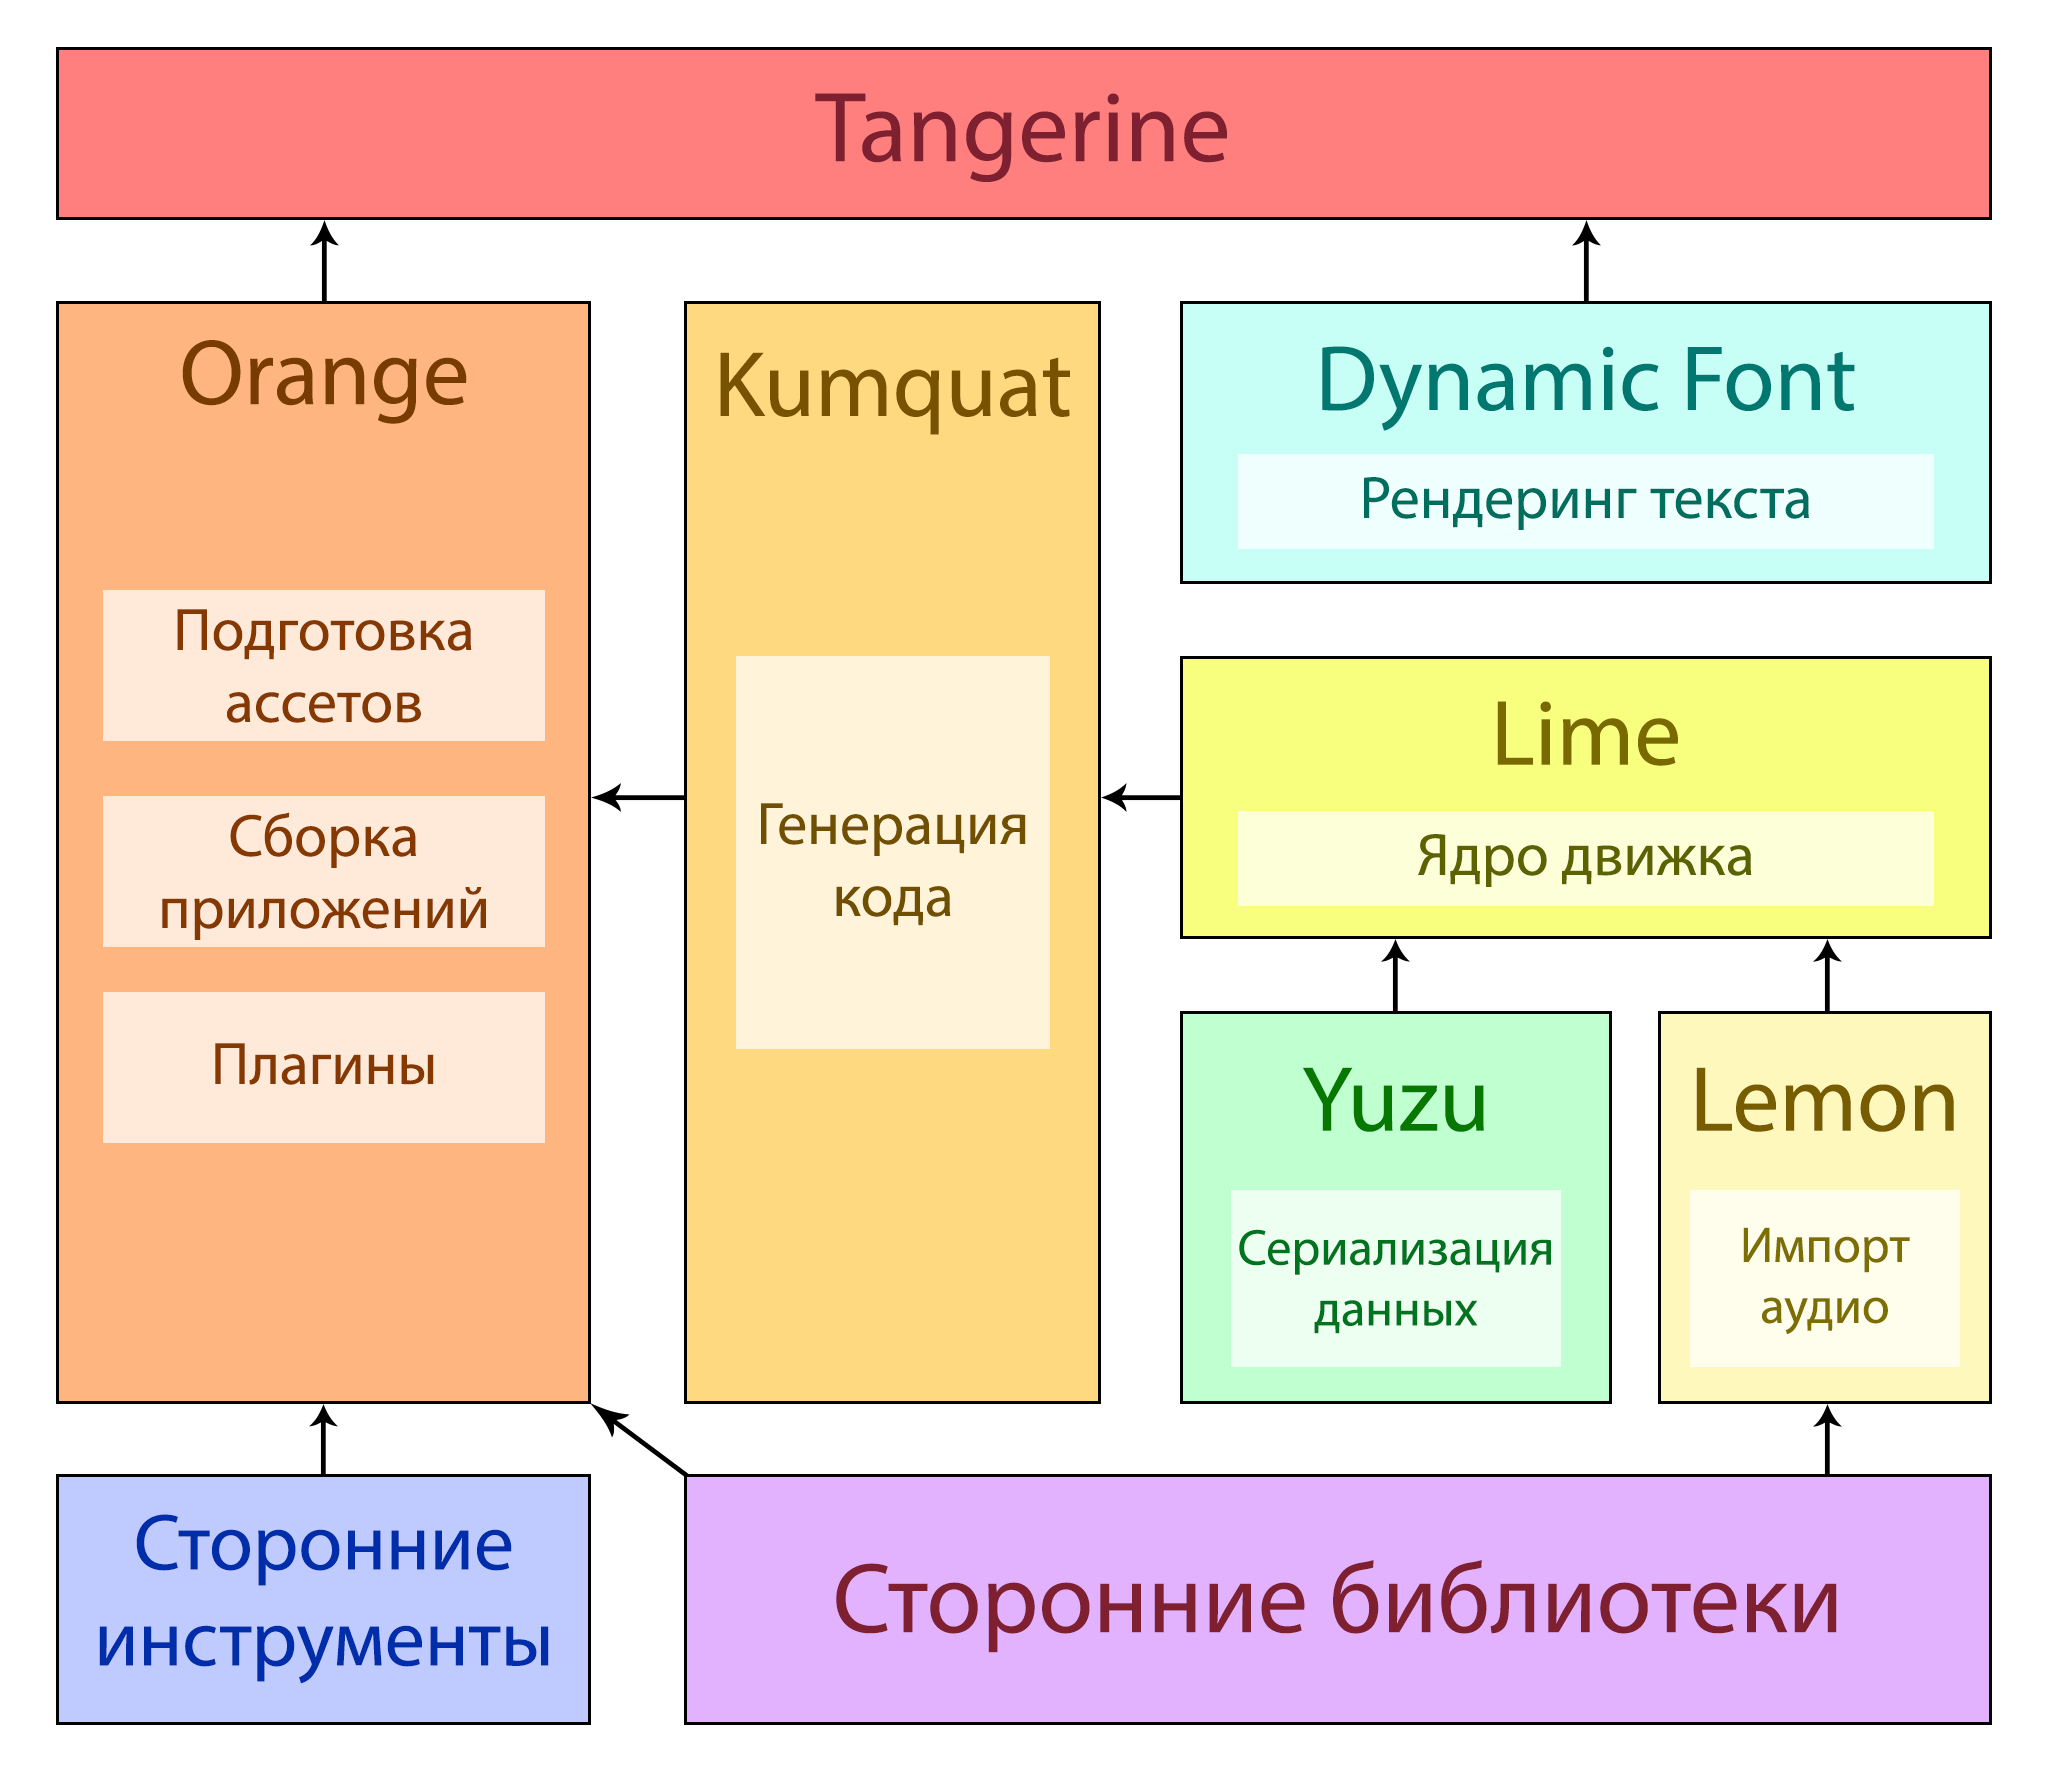
\includegraphics[width=1\linewidth]{images/CitrusScheme.png}
					\caption{Схема модулей движка Citrus}
					\label{img:CitrusScheme}
				\end{figure}
				%\par \textbf{Добавить огромное количество инфы про цитрус}
			\subsubsection{Текстовый редактор}
				\par Текстовый редактор это компьютерная программа (или её часть), 
				предназначенная для создания и изменения текстовых данных (в том числе 
				текстовых файлов). Часто редакторы предоставляют пользователям дополнительные 
				возможности, такие как: копирование и вставка, поиск и замена текста, 
				форматирование текста (переносы строк, выравнивание и пр.), 
				откат/восстановление изменений \cite{WhatIsATextEditor}. 
				\par Некоторые редакторы, помимо работы с обычным текстом, позволяют также и
				работу со стилизованным текстом (т.н. Rich Text) 
				\cite{DiffBetweenTextFormats}. Так как текстовый формат данных не предполагает
				хранения информации о стиле текста, в редакторах тексты обрамляются в различные
				языки разметки (например, HTML), либо используется внутреннее двоичное 
				представление.
				\par Для успешной работы текстового редактора необходимо, чтобы были
				реализованы три его основные компоненты: \cite{CraftOfTextEditing}
				\begin{enumerate}
					\item Обработка внутреннего представления текста --- текст необходимо
					эффективным образом хранить и изменять, наивный подход к этой части
					редактора приведёт к значительному (в случае работы с большими объемами
					данных -- к фатальному) падению производительности всего редактора.
					\item Отрисовка --- текст необходимо правильно отрисовать с учетом размеров
					окна и применённых стилей (шрифт, выравнивание, переносы слов).
					\item Обработка пользовательского ввода --- приём команд
					(вставка, удаление элемента, перевод курсора и~пр.) и передача их
					обработчику внутреннего представления.
				\end{enumerate}
			\subsubsection{Обработка текста в Citrus}
				\par Представление текстовых данных и работа с ними -- важная часть игрового
				движка, поскольку значительная часть важной игровой информации сообщается 
				пользователю в текстовом виде. 
				%\textbf{Вставить инфу о классах, занимающихся
				%текстом (IText, RichText, SimpleText, TextParser, TextStyle, TextRenderer,
				%Editor)} 
				В Citrus есть классы, обеспечивающие обработку ввода и отрисовку текста, 
				однако они реализованы неэффективно, что выражается в резком падении 
				производительности с увеличением длины текста. Это приводит к увеличению
				требований к процессору для поддержания высокой частоты кадров. При дальнейшем
				увеличении объема текста работа программ сильно замедляется, что критично для
				игровых проектов, и составляет значительные неудобства при работе со средствами
				визуального редактирования в движке. Также стоит отметить, что несмотря на
				возможность корректно отображать многострочный текст, текущая система слабо
				приспособлена для его редактирования.
				\par В данный момент эти проблемы решаются обходным путём, т.е. число
				использований многострочного редактора сведено к минимуму, а появления больших
				объемов текста стараются, по возможности, не допускать. В игровых проектах
				число больших текстов невелико, а во время работы с визуальной частью движка
				неэффективность работы текстовой системы, хоть и замедляет работу, не является
				критическим препятствием.
				\par Для решения данных проблем можно переписать всю систему работы с текстом с
				нуля, а можно лишь оптимизировать малоэффективные части. Поскольку разработка 
				подобной системы связана со значительными трудностями, в то время как на уже
				существующую систему опираются многие игровые проекты, я решил лишь внести 
				необходимые изменения в существующую структуру работы.
				\par Первую часть системы -- обработку внутреннего представления текста -- 
				можно использовать как самостоятельную единицу в любых других проектах. Все 
				прочие части завязаны на существующую архитектуру движка Citrus и без него 
				неприменимы.
		\subsection{Неформальная постановка задачи}
			В рамках данной работы требуется выполнить следующие задачи:
			\begin{enumerate}
				\item Изучить имеющиеся подходы к реализации текстовых редакторов
				\item Создать редактор, обеспечивающий:
				\begin{itemize}
					\setlength{\itemindent}{-3em}
					\item Просмотр и редактирование обычного (не стилизованного) текста
					\item Поддержку работы с многострочными файлами
					\item Эффективную отрисовку больших объемов текста
					\item Поддержку стандартных пользовательских команд
				\end{itemize}
				\item Сравнить производительность новой и старой версий редактора
			\end{enumerate}
		\subsection{План работ}
			\begin{itemize}
				\item Изучение подходов к реализации текстовых редакторов (1-2 недели)
				\item Изучение кодовой базы движка Citrus в целях нахождения места для внесения
				изменений (1 неделя)
				\item Реализация текстового редактора (4 недели)
				\item Подготовка отчёта (1 неделя)
			\end{itemize}
	\section{Обзор существующих методов решения}
		\subsection{Внутреннее представление текста}
			\par Для хранения и обработки текстовых данных используются различные подходы,
				хотя общее число зарекомендовавших себя относительно невелико.
				\cite{TextEditorDataStructures}.
			\par Для работы текстового редактора любая из структур должна поддерживать, как 
			минимум, следующие операции: вставку и удаление символов, получение элемента по его
			номеру, получение элемента по строке и столбцу.
			\subsubsection{Массив символов}
				\par Наиболее очевидный способ хранения текста. Вся текстовая информация
				располагается в одном массиве. Это накладывает большие ограничения на скорость
				удаления и вставки \cite{StringsReference}. 
				\par Для удаления необходимо сдвинуть все элементы массива, начиная с позиции
				последнего удаляемого элемента, влево на число позиций, равное размеру
				удаляемой последовательности. Для вставки нужно сдвинуть все элементы, начиная
				с позиции вставки, вправо на число позиций, равное размеру удаляемой
				последовательности, а затем вставить последовательность в позицию вставки.
				\par Алгоритмическая сложность удаления и вставки -- $O(n)$. Учитывая 
				количество символов, зачастую присутствующее в тексте, это чудовищно плохой 
				показатель.
				\par Сложность получения элемента по номеру -- $O(1)$, поскольку достаточно
				применить адресную арифметику. В то же время, сложность получения элемента по
				строке и столбцу -- $O(n)$, потому что необходимо пробежаться по всем элементам
				массива, подсчитывая количество строк, до момента достижения необходимой
				позиции.
				\par Несмотря на недостаточную эффективность, у подхода есть одно преимущество
				-- его очень легко реализовать. Однако для реализации чего-либо кроме
				простейшего однострочного поля ввода стоит предпочесть другие варианты.
			\subsubsection{Буферное окно (Gap buffer)}
				\par Текст хранится в массиве, однако часть строки не заполнена и служит для
				заполнения в случае необходимости вставки элемента. Так как в текстовых
				редакторах изменения, зачастую, происходят около одного места (позиция 
				курсора), то операции вставки и удаления можно выполнять очень быстро.
				Узким местом подхода является тот факт, что при интенсивных вставках элементов
				буфер может закончиться, в этом случае его необходимо будет расширить заново,
				выполнив операцию сдвига всех элементов вправо с определенной позиции на размер
				буфера. Перемещение буфера к позиции курсора так же требует времени, в худшем 
				случае (курсор переместили от начала текста к его концу) необходимо сдвинуть
				все элементы в массиве \cite{GapBufferArticle}.
				\par Факт эффективности подхода основан на предположении, что стоимость
				перемещения курсора и расширения буфера амортизируется с помощью прочих,
				дешевых операций, поскольку операции перемещения курсора и расширения буфера
				довольно редки по сравнению с операциями вставки.
				\par Алгоритмическая сложность удаления и вставки, в худшем случае, $O(n)$. Для
				данного подхода затруднительно оценить среднестатистическую сложность.
				\par Сложность получения элемента по индексу, как и в случае с обычным 
				массивом, $O(1)$, адресная арифметика всё так же применима при условии, что
				текущий размер буфера всегда известен. Сложность получения элемента по строке и
				столбцу, по тем же причинам, что и у обычного массива, составляет $O(n)$.
				\par Данный подход легко реализуем и даёт значительный прирост
				производительности по сравнению с использованием обычного массива, однако он не
				рассчитан на работу с большими файлами, поскольку в них стоимость операций 
				перемещения курсора и расширения буфера чрезвычайно высоки.
				\par Тем не менее, данный подход нашел применение во многих текстовых
				редакторах, в том числе в весьма известных (например, Emacs
				\cite{EmacsGapBuffer}). %\textbf{Если близко, то быстро}
				\par Пример работы. Исходное состояние:
				$$Lorem~ipsum~dolor~sit~[~~~~~~~~~~~~]~adipiscing.$$
				\par Пользователь добавляет текст:
				$$Lorem~ipsum~dolor~sit~amet,[~~]~adipiscing.$$
				\par Пользователь перемещает курсор
				$$Lorem~ipsum~dolor~sit~[~~]~amet,~adipiscing.$$
				\par Пользователь добавляет текст, полностью заполняющий буфер. Система
				расширяет буфер:
				$$Lorem~ipsum~dolor~sit~consectetur[~~~~~~~~~~]~amet,~adipiscing.$$
			\subsubsection{Связный список}
				\par Элементы (например, символы) хранятся в узлах односвязного списка. При 
				таком подходе операции вставки и удаления выполняются очень быстро, поскольку 
				сводятся к манипуляциям с указателями. Проблемой в данном случае становится 
				операция получения элемента по некоторому индексу, поскольку необходимо пройти 
				по указателям от начала и до требуемого элемента, что в худшем случае занимает 
				$O(n)$ времени (для получения элемента по номерам строки и столбца сложность та
				же), причём эту операцию требуется выполнить и для вставки или удаления 
				элементов. Помимо прочего, на хранение большого числа узлов требуется 
				колоссальный объем памяти, поскольку в одном узле хранится лишь по одному 
				символу \cite{LinkedListReference}. 
				\par Преимуществом этого подхода является тот факт, что в узлах, помимо
				информации о символе, можно хранить и прочую информацию, например, информацию
				о стиле текста.
			\subsubsection{Набор строк}
				\par Предыдущие варианты реализации текстовых редакторов не ориентированы на
				применение в многострочных редакторах. Использование набора строк --
				естественное решение этой проблемы. Текст представляется в виде набора
				массивов, каждый из которых хранит только по одной строке текста. Стоит
				отметить, что вместо обычных массивов можно использовать описанные выше
				подходы для увеличения эффективности. Использование набора строк позволяет
				оптимизировать отрисовку. Зная номера строк, в данный момент помещающихся в 
				активное окно, можно быстро к ним обратиться и отрисовать только строго
				необходимый объем текста. 
				\par Этот подход раскрывается при использовании в многострочных редакторах,
				поскольку позволяет за $O(1)$ обращаться к элементам по номерам строки и
				столбца.
			%\subsubsection{Верёвка (Rope)}
			%	\par \textbf{Потом вставить}
			\subsubsection{Таблица кусочков (Piece Table)}
				\par Эффективная структура данных, используемая во многих современных 
				текстовых редакторах \cite{PieceTableArticle}. Используется несколько потоков
				(файлов) -- исходный и добавочный. Исходный поток используется только для 
				чтения. В добавочный данные добавляются и читаются из него, но не удаляются.
				Вместо хранения самих символов, в структуре хранится информация о текстовых 
				фрагментах, а именно: позиция начала фрагмента в потоке (файле), его длина, 
				исходный ли это поток или добавочный. При добавлении новых символов они
				записываются в добавочный поток, а в таблицу заносится новый фрагмент. При
				вставке текста, в случае если позиция нового фрагмента содержится внутри
				существующего, возможно разбиение фрагментов на две части, тогда в левой части
				фрагмента остаётся информация о части текста, лежащей до нового фрагмента, а в 
				правой -- после. Во время удаления от фрагментов "отрезаются" части, либо весь
				фрагмент удаляется целиком.
				\par Таблица кусочков это лишь структура данных для хранения информации о
				тексте, настоящую эффективность данному подходу придаёт способ хранения
				кусочков. Одним из наиболее эффективных способов является использование 
				расширяющегося дерева (Splay Tree). Это сбалансированное бинарное дерево 
				поиска, в котором элементы, к которым в последний раз было произведено
				обращение, перемещаются в корень. Это свойство особенно эффективно при
				использовании в текстовых редакторах, поскольку в них большая часть изменений
				производится около одного места -- позиции курсора \cite{SplayTreeArticle}.
				\par При использовании расширяющегося дерева сложность вставки и удаления
				составляет $O(log~m)$, где $m$ -- число фрагментов в дереве. Операция получения
				элемента так же выполняется за $O(log~m)$, однако стоит учесть, что
				требуются дополнительные затраты времени на чтение данных из потока.
				\par Операция получения элемента по номерам строки и столбца в случае наивной
				реализации имеет сложность $O(n)$, где $n$ -- число символов в тексте, однако
				зачастую применяются различные техники для оптимизации этой операции.
				\par Все вышеперечисленные сложности описаны для худшего случая, в случае
				работы с текстом в позиции курсора операции будут выполнены значительно 
				быстрее, поскольку все необходимые элементы будут находиться близко к корню
				дерева, благодаря чему для достижения нужной позиции не потребуется совершать
				полный пробег по дереву.
				\par Дополнительным преимуществом подхода является тот факт, что он
				использует значительно меньше памяти, чем прочие, поскольку вместо хранения,
				непосредственно, символов, хранится лишь набор ссылок на части текста.
				%\textbf{Вставить картинку}
			\subsubsection{Сравнение}
				\par{Для наглядности построим сравнительную таблицу (см. Табл. 
				\ref{table:MethodComplexity})}
				\begin{table}[h]
					\begin{center}
						\begin{tabular}{|*{5}{p{3cm}|}}
							\hline
							Подход & Вставка & Удаление & Обращение по номеру & Обращение по 
							номеру строки и столбца \\
							\hline
							Массив & $O(n)$ & $O(n)$ & $O(1)$ & $O(n)$ \\
							\hline
							Буферное окно & $O(n)$ & $O(n)$ & $O(1)$ & $O(n)$ \\
							\hline
							Связный список & $O(n)$ & $O(n)$ & $O(n)$ & $O(n)$ \\
							\hline
							Набор строк & $O(n)$ & $O(n)$ & $O(1)$ & $O(1)$ \\
							\hline
							Таблица кусочков & $O(log~m)$ & $O(log~m)$ & $O(log~m)$ & $O(n)$ \\
							\hline
						\end{tabular}
						\caption{Сравнение алгоритмических сложностей подходов}
						\label{table:MethodComplexity}
					\end{center}
				\end{table}
				\par К сожалению, для многих подходов трудно вывести алгоритмическую сложность
				в среднем случае, многое зависит от ряда оговорок и условий работы. Тем не
				менее, учитывая описанные выше особенности подходов, можно с уверенностью
				утверждать, что таблица кусочков -- это наиболее эффективный способ организации
				внутреннего представления текста.
	\section{Требования к окружению}
		\subsection{Требования к аппаратному обеспечению}
			\par Поскольку текстовый редактор является частью движка Citrus и не существует 
			без него, то ниже приведены общие требования для запуска движка и игровых проектов,
			сделанных на его основе.
			\begin{itemize}
				\item GPU с поддержкой OpenGL ES 2.0 либо Vulkan либо Molten VK
				\item CPU с частотой 1 ГГц или выше
				\item 512 Мб RAM или больше
			\end{itemize}
		\subsection{Требования к программному обеспечению}
			\par Поскольку текстовый редактор является частью движка Citrus и не существует 
			без него, то ниже приведены общие требования для запуска движка и игровых проектов,
			сделанных на его основе.
			\begin{itemize}
				\item ОС Windows 8.1 или выше; macOS 10.13 или выше; дистрибутивы 
				Linux, поддерживающие среду Mono; Android 5 или выше; iOS 10.3.3 или выше
				\item .NET Framework версии 4.7.1 или выше
			\end{itemize}
	\section{Архитектура системы}
		\par Систему можно поделить на три модуля:
		\begin{enumerate}
			\item Модуль обработки внутреннего представления текста --- отвечает за хранение
			текста и эффективное выполнение базовых операций (вставка, удаление, доступ).
			\item Модуль отрисовки --- обеспечивает корректную и эффективную отрисовку текста
			с учетом размеров виджета.
			\item Модуль обработки пользовательского ввода --- отвечает за получение
			пользовательских команд и отправку их в обработчик внутреннего представления.
		\end{enumerate}
	\section{Спецификация данных}
		\subsection{Описание формата или структуры данных}
			\par Данная реализация текстового редактора не предполагает поддержку
			стилизованного текста, однако подобная функциональность заложена в архитектуру.
			Для указания информации о стиле будут использоваться тэги, подобные тем, что
			используются в HTML.
	\section{Функциональные требования}
		\par Модуль обработки внутреннего представления текста должен уметь:
		\begin{itemize}
			\item Хранить текст
			\item Вставлять текстовую строку в позицию курсора (\textit{Здесь и далее под текстовой позицией 
			понимается номер элемента, перед которым будет применена операция, под
			позицией курсора понимаются номера строки и столбца, на которые в данный момент
			ссылается курсор}).
			\item Удалять текстовый фрагмент определённого размера, 
			начиная с позиции курсора.
			\item Выделять текстовый фрагмент определённого размера.
			\item Удалять предыдущий/следующий за курсором символ.
			\item Перемещать курсор на позицию предыдущего/следующего
			за курсором элемента.
			\item Перемещать курсор в начало / конец текущей строки
			\item Перемещать курсор на строку вверх/вниз.
			\item Перемещать курсор на определенную текстовую позицию.
			\item Расширять/сужать выделение на предыдущий/следующий за курсором элемент.
			\item Копировать, вырезать и, впоследствии, вставлять выделенный текстовый 
			фрагмент.
			\item Отменять предыдущую выполненную операцию.
			\item Повторно выполнять предыдущую отмененную операцию.
			\item Получать вест текущий текст в формате текстовой 
			строки.
		\end{itemize}
		\par Модуль отрисовки должен:
		\begin{itemize}
			\item Выполнять отрисовку текста в заданном окне в рамках прямоугольной области, 
			параметры которой задаются программистом, с учетом параметров шрифта.
			\item Обеспечивать перенос слов на следующую строку, в случае, если
			текущая строка по горизонтали не помещается в видимую область, при условии, что 
			данный режим переноса активирован (soft wrap).
			\item Отрисовывать только видимую часть текста, отбрасывая строки, в данный момент
			не попадающие в видимую область
			\item Обеспечивать возможность вертикальной и/или горизонтальной прокрутки 
			текста
			\item Выполнять отрисовку курсора в его текущей позиции
		\end{itemize}
		\par Модуль обработки пользовательского ввода должен:
		\begin{itemize}
			\item Обрабатывать ввод текстовых данных с клавиатуры
			\item Обрабатывать нажатия на клавиши стрелок 
			("Вверх", "Вниз", "Влево", "Вправо").
			\item Обрабатывать клики мышью / касание экрана по/в области отрисовки текста.
			\item Обрабатывать клик мышью и протягивание / касание экрана и протягивание по 
			области отрисовки текста.
			\item Обрабатывать нажатия на клавиши "Home" и "End"
			\item Обрабатывать нажатия на комбинации "Shift + Влево", "Shift + Вправо", 
			"Shift + Вниз", "Shift + Вверх", "Shift + Home", "Shift + End"
			\item Обрабатывать нажатия на клавиши "Backspace" и "Delete"
			\item Обрабатывать вызов контекстного меню и выбор в нём действия (способ вызова
			меню зависит от платформы, так, для ПК, способом вызова меню является клик правой
			кнопкой мыши по области редактора)
		\end{itemize}
		%\textbf{Enter и ctrl}
	\section{Требования к интерфейсу}
		\par Текстовый редактор предназначен для оконных интерфейсов. Интерфейс представляет
		собой прямоугольник в заданной области окна, внутри которого рисуется текст и курсор. Окно редактора может обладать 
		вертикальным скроллбаром, горизонтальным или никаким. Для взаимодействия с редактором
		используются клавиши клавиатуры, 
		аппаратной или электронной, действия контекстного меню, клики мыши/касания экрана.
		\par Текст может рисоваться с применением разных настроек шрифта, с использованием soft
		wrap или без него.
	\section{Прочие требования}
		\subsection{Требования к производительности}
			Вся цепочка операций (от обработки изменений текста до 
			отрисовки) должна выполняться не более чем за 30 миллисекунд (для отрисовки 30 
			кадров в секунду) для многострочных файлов порядка нескольких мегабайт на экранах
			разрешением порядка 1024x768. %\textbf{Убедиться}
	\section{Проект}
		\subsection{Средства реализации}
			Все части системы были реализованы на языке C\# 7.0, 
			версия .NET Framework 4.7.1, поскольку это стандарт для компании Game Forest.
		\subsection{Структуры данных}
			\begin{itemize}
				\item PieceTreeNode --- узел расширяющегося дерева, хранит информацию о 
				текстовых фрагментах: поток, в котором находится фрагмент (исходный или
				добавочный), позиция фрагмента в потоке, его длина, позиция в итоговом 
				тексте, ссылки на родителя и потомков
				\item PieceTree --- расширяющееся дерево, узлами в котором являются
				PieceTreeNode. В нём выполняются все операции балансировки дерева, поиска,
				вставки, удаления элементов, а так же операции undo и redo
				\item Word --- структура для хранения информации об отдельном слове, включает в
				себя индекс слова в массиве слов, ширину, горизонтальную позицию, нужно ли
				вставить перенос строки перед словом
				\item Line --- структура для хранения информации о строках текста, включает
				общую ширину и высоту строки, номер первого слова в массиве слов, входящего в
				строку, число слов
			\end{itemize}
		\subsection{Модули и алгоритмы}
			\subsubsection{Обработка внутреннего представления текста}
				\par Данный модуль состоит из следующих классов:
				\begin{itemize}
					\item CaretPosition --- описывает положение курсора и 
					обрабатывает его перемещение.
					\item Selection --- хранит информацию о текущем выделении, обрабатывает его
					изменения
					\item UndoStack --- хранит стек обработанных операций, по запросу PieceTree 
					сообщает необходимые данные 
					\item SubEditor --- связующее звено между модулями. Принимает команды на 
					редактирование текста и перемещение курсора, перенаправляет их
					соответствующим модулям
				\end{itemize}
			\subsubsection{Модуль отрисовки}
				\par Данный модуль состоит из следующих классов:
				\begin{itemize}
					\item TextParser --- выделяет из текста фрагменты (отдельные слова, 
					переносы строк, пробелы)
					\item TextRenderer --- получает набор фрагментов от TextParser, для каждого
					фрагмента определяет его позицию в тексте, учитывая параметры шрифта и 
					размеры окна, при необходимости применяет soft wrap, затем передаёт
					полученные данные в общий рендерер движка, который выполняет
					непосредственную отрисовку
					\item CommonText --- содержит в себе SubEditor, TextParser и TextRenderer,
					обеспечивает обмен данными между ними, помимо этого содержит информацию о
					параметрах шрифта. Стоит отметить, что в случаях, когда необходимо лишь 
					отобразить текст без возможности редактирования, достаточно возможностей
					этого класса
				\end{itemize}
			\subsubsection{Модуль обработки пользовательского ввода}
				\par Вся функциональность данного модуля содержится в классе Editor. Он
				обрабатывает пользовательский ввод, перенаправляя команды в SubEditor,
				находящийся внутри CommonText, который является полем в Editor.
				%\textbf{В доме, который построил Джек. Надо бы перефразировать.}
		\subsection{Проблемы и решения}
			\par В ходе разработки пришлось столкнуться со следующими проблемами:
			\begin{itemize}
				\item Выбор структуры данных вызвал затруднения, поскольку необходимо было
				соблюсти баланс между эффективностью и сложностью разработки. Тем не менее,
				было принято решение использовать наиболее эффективный подход, несмотря на 
				потенциальные сложности при реализации.
				\item Текущая архитектура не позволяла проводить тестирование скорости 
				прокрутки, поскольку она всегда рисовала виджет целиком и показывала лишь 
				видимую его часть, что в корне противоречит идее оптимизации. Было принято
				решение написать новый класс на основе старого, позволяющий отрисовывать только
				видимую часть текста и не тратить ресурсы на остальную.
			\end{itemize}
		\subsection{Стандарт кодирования}
			Использован стандарт кодирования, принятый в Game Forest \cite{CodingConventions}.
		%\subsection{Проект интерфейса}
		%	\textbf{Можно вставить скрины CommonText, ScrollView и Editor}
	\section{Реализация и тестирование}
		\par Объем кода: 3338 строк, ~140 кб
		\par Число коммитов: 46
		\par Количество автотестов: 63
		\par Репозиторий: https://github.com/mrojkov/Citrus
		%\textbf{Родить акт о внедрении}
		\subsection{Вычислительный эксперимент}
			\par Было проведено ручное сравнение производительности предыдущей и новой версий 
			редактора. Тестирование проводилось на тексте объемом 100 тысяч строк.
			\par Тестирование показало, что при вертикальной прокрутке новый вариант редактора
			редактора отрисовывает текст без задержки на высокой частоте кадров, в то время как
			старая версия показывает новый кадр с задержкой в 2-3 секунды.
	\section*{Заключение}
		\par Таким образом, в процессе выпускной квалификационной работы:
		\begin{itemize}
			\item Были исследованы подходы к реализации текстовых редакторов
			\item Был реализован текстовый редактор для open-source движка Citrus
		\end{itemize}
		\par Были углублены знания в области:
		\begin{itemize}
			\item Языка программирования C\#
			\item Реализации текстовых редакторов
			\item Проектирования система
			\item Работы с системами контроля версий
			\item Внутренних процессов компании Game Forest
		\end{itemize}
		\par Новый текстовый редактор поддерживает работу с многострочными файлами и работает
		значительно быстрее, чем предыдущий.
		\par В рамках дальнейшего развития можно реализовать поддержку стилизованного текста,
		а так же переосмыслить архитектуру модуля отрисовки для упрощения кода.
	\newpage
	\bibliographystyle{ugost2008ls}
	\bibliography{references}	
\end{document}